\documentclass[1p]{elsarticle_modified}
%\bibliographystyle{elsarticle-num}

%\usepackage[colorlinks]{hyperref}
%\usepackage{abbrmath_seonhwa} %\Abb, \Ascr, \Acal ,\Abf, \Afrak
\usepackage{amsfonts}
\usepackage{amssymb}
\usepackage{amsmath}
\usepackage{amsthm}
\usepackage{scalefnt}
\usepackage{amsbsy}
\usepackage{kotex}
\usepackage{caption}
\usepackage{subfig}
\usepackage{color}
\usepackage{graphicx}
\usepackage{xcolor} %% white, black, red, green, blue, cyan, magenta, yellow
\usepackage{float}
\usepackage{setspace}
\usepackage{hyperref}

\usepackage{tikz}
\usetikzlibrary{arrows}

\usepackage{multirow}
\usepackage{array} % fixed length table
\usepackage{hhline}

%%%%%%%%%%%%%%%%%%%%%
\makeatletter
\renewcommand*\env@matrix[1][\arraystretch]{%
	\edef\arraystretch{#1}%
	\hskip -\arraycolsep
	\let\@ifnextchar\new@ifnextchar
	\array{*\c@MaxMatrixCols c}}
\makeatother %https://tex.stackexchange.com/questions/14071/how-can-i-increase-the-line-spacing-in-a-matrix
%%%%%%%%%%%%%%%

\usepackage[normalem]{ulem}

\newcommand{\msout}[1]{\ifmmode\text{\sout{\ensuremath{#1}}}\else\sout{#1}\fi}
%SOURCE: \msout is \stkout macro in https://tex.stackexchange.com/questions/20609/strikeout-in-math-mode

\newcommand{\cancel}[1]{
	\ifmmode
	{\color{red}\msout{#1}}
	\else
	{\color{red}\sout{#1}}
	\fi
}

\newcommand{\add}[1]{
	{\color{blue}\uwave{#1}}
}

\newcommand{\replace}[2]{
	\ifmmode
	{\color{red}\msout{#1}}{\color{blue}\uwave{#2}}
	\else
	{\color{red}\sout{#1}}{\color{blue}\uwave{#2}}
	\fi
}

\newcommand{\Sol}{\mathcal{S}} %segment
\newcommand{\D}{D} %diagram
\newcommand{\A}{\mathcal{A}} %arc


%%%%%%%%%%%%%%%%%%%%%%%%%%%%%5 test

\def\sl{\operatorname{\textup{SL}}(2,\Cbb)}
\def\psl{\operatorname{\textup{PSL}}(2,\Cbb)}
\def\quan{\mkern 1mu \triangleright \mkern 1mu}

\theoremstyle{definition}
\newtheorem{thm}{Theorem}[section]
\newtheorem{prop}[thm]{Proposition}
\newtheorem{lem}[thm]{Lemma}
\newtheorem{ques}[thm]{Question}
\newtheorem{cor}[thm]{Corollary}
\newtheorem{defn}[thm]{Definition}
\newtheorem{exam}[thm]{Example}
\newtheorem{rmk}[thm]{Remark}
\newtheorem{alg}[thm]{Algorithm}

\newcommand{\I}{\sqrt{-1}}
\begin{document}

%\begin{frontmatter}
%
%\title{Boundary parabolic representations of knots up to 8 crossings}
%
%%% Group authors per affiliation:
%\author{Yunhi Cho} 
%\address{Department of Mathematics, University of Seoul, Seoul, Korea}
%\ead{yhcho@uos.ac.kr}
%
%
%\author{Seonhwa Kim} %\fnref{s_kim}}
%\address{Center for Geometry and Physics, Institute for Basic Science, Pohang, 37673, Korea}
%\ead{ryeona17@ibs.re.kr}
%
%\author{Hyuk Kim}
%\address{Department of Mathematical Sciences, Seoul National University, Seoul 08826, Korea}
%\ead{hyukkim@snu.ac.kr}
%
%\author{Seokbeom Yoon}
%\address{Department of Mathematical Sciences, Seoul National University, Seoul, 08826,  Korea}
%\ead{sbyoon15@snu.ac.kr}
%
%\begin{abstract}
%We find all boundary parabolic representation of knots up to 8 crossings.
%
%\end{abstract}
%\begin{keyword}
%    \MSC[2010] 57M25 
%\end{keyword}
%
%\end{frontmatter}

%\linenumbers
%\tableofcontents
%
\newcommand\colored[1]{\textcolor{white}{\rule[-0.35ex]{0.8em}{1.4ex}}\kern-0.8em\color{red} #1}%
%\newcommand\colored[1]{\textcolor{white}{ #1}\kern-2.17ex	\textcolor{white}{ #1}\kern-1.81ex	\textcolor{white}{ #1}\kern-2.15ex\color{red}#1	}

{\Large $\underline{12n_{0283}~(K12n_{0283})}$}

\setlength{\tabcolsep}{10pt}
\renewcommand{\arraystretch}{1.6}
\vspace{1cm}\begin{tabular}{m{100pt}>{\centering\arraybackslash}m{274pt}}
\multirow{5}{120pt}{
	\centering
	\includegraphics[width=112pt]{../../../GIT/diagram.site/Diagrams/png/2372_12n_0283.png}\\
\ \ \ A knot diagram\footnotemark}&
\allowdisplaybreaks
\textbf{Linearized knot diagam} \\
\cline{2-2}
 &
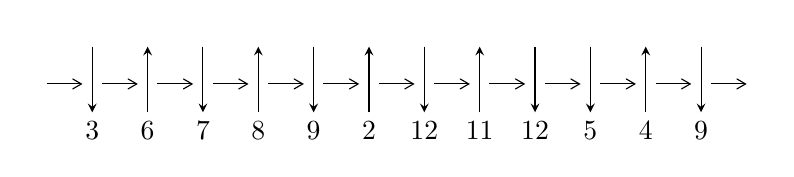
\begin{tikzpicture}[x=20pt, y=17pt]
	% nodes
	\node (C0) at (0, 0) {};
	\node (C1) at (1, 0) {};
	\node (C1U) at (1, +1) {};
	\node (C1D) at (1, -1) {3};

	\node (C2) at (2, 0) {};
	\node (C2U) at (2, +1) {};
	\node (C2D) at (2, -1) {6};

	\node (C3) at (3, 0) {};
	\node (C3U) at (3, +1) {};
	\node (C3D) at (3, -1) {7};

	\node (C4) at (4, 0) {};
	\node (C4U) at (4, +1) {};
	\node (C4D) at (4, -1) {8};

	\node (C5) at (5, 0) {};
	\node (C5U) at (5, +1) {};
	\node (C5D) at (5, -1) {9};

	\node (C6) at (6, 0) {};
	\node (C6U) at (6, +1) {};
	\node (C6D) at (6, -1) {2};

	\node (C7) at (7, 0) {};
	\node (C7U) at (7, +1) {};
	\node (C7D) at (7, -1) {12};

	\node (C8) at (8, 0) {};
	\node (C8U) at (8, +1) {};
	\node (C8D) at (8, -1) {11};

	\node (C9) at (9, 0) {};
	\node (C9U) at (9, +1) {};
	\node (C9D) at (9, -1) {12};

	\node (C10) at (10, 0) {};
	\node (C10U) at (10, +1) {};
	\node (C10D) at (10, -1) {5};

	\node (C11) at (11, 0) {};
	\node (C11U) at (11, +1) {};
	\node (C11D) at (11, -1) {4};

	\node (C12) at (12, 0) {};
	\node (C12U) at (12, +1) {};
	\node (C12D) at (12, -1) {9};
	\node (C13) at (13, 0) {};

	% arrows
	\draw[->,>={angle 60}]
	(C0) edge (C1) (C1) edge (C2) (C2) edge (C3) (C3) edge (C4) (C4) edge (C5) (C5) edge (C6) (C6) edge (C7) (C7) edge (C8) (C8) edge (C9) (C9) edge (C10) (C10) edge (C11) (C11) edge (C12) (C12) edge (C13) ;	\draw[->,>=stealth]
	(C1U) edge (C1D) (C2D) edge (C2U) (C3U) edge (C3D) (C4D) edge (C4U) (C5U) edge (C5D) (C6D) edge (C6U) (C7U) edge (C7D) (C8D) edge (C8U) (C9U) edge (C9D) (C10U) edge (C10D) (C11D) edge (C11U) (C12U) edge (C12D) ;
	\end{tikzpicture} \\
\hhline{~~} \\& 
\textbf{Solving Sequence} \\ \cline{2-2} 
 &
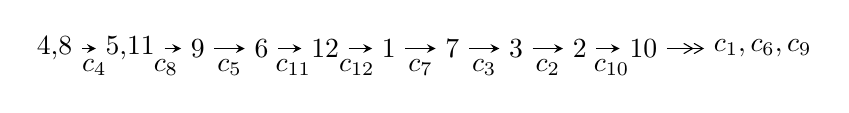
\begin{tikzpicture}[x=23pt, y=7pt]
	% node
	\node (A0) at (-1/8, 0) {4,8};
	\node (A1) at (17/16, 0) {5,11};
	\node (A2) at (17/8, 0) {9};
	\node (A3) at (25/8, 0) {6};
	\node (A4) at (33/8, 0) {12};
	\node (A5) at (41/8, 0) {1};
	\node (A6) at (49/8, 0) {7};
	\node (A7) at (57/8, 0) {3};
	\node (A8) at (65/8, 0) {2};
	\node (A9) at (73/8, 0) {10};
	\node (C1) at (1/2, -1) {$c_{4}$};
	\node (C2) at (13/8, -1) {$c_{8}$};
	\node (C3) at (21/8, -1) {$c_{5}$};
	\node (C4) at (29/8, -1) {$c_{11}$};
	\node (C5) at (37/8, -1) {$c_{12}$};
	\node (C6) at (45/8, -1) {$c_{7}$};
	\node (C7) at (53/8, -1) {$c_{3}$};
	\node (C8) at (61/8, -1) {$c_{2}$};
	\node (C9) at (69/8, -1) {$c_{10}$};
	\node (A10) at (11, 0) {$c_{1},c_{6},c_{9}$};

	% edge
	\draw[->,>=stealth]	
	(A0) edge (A1) (A1) edge (A2) (A2) edge (A3) (A3) edge (A4) (A4) edge (A5) (A5) edge (A6) (A6) edge (A7) (A7) edge (A8) (A8) edge (A9) ;
	\draw[->>,>={angle 60}]	
	(A9) edge (A10);
\end{tikzpicture} \\ 

\end{tabular} \\

\footnotetext{
The image of knot diagram is generated by the software ``\textbf{Draw programme}" developed by Andrew Bartholomew(\url{http://www.layer8.co.uk/maths/draw/index.htm\#Running-draw}), where we modified some parts for our purpose(\url{https://github.com/CATsTAILs/LinksPainter}).
}\phantom \\ \newline 
\centering \textbf{Ideals for irreducible components\footnotemark of $X_{\text{par}}$} 
 
\begin{align*}
I^u_{1}&=\langle 
b- u,\;-3.85888\times10^{16} u^{31}+4.26003\times10^{16} u^{30}+\cdots+3.07647\times10^{15} a-2.04981\times10^{16},\\
\phantom{I^u_{1}}&\phantom{= \langle  }u^{32}- u^{31}+\cdots+13 u^2+1\rangle \\
I^u_{2}&=\langle 
b+u,\;3 u^{16}-3 u^{15}+\cdots+a-1,\\
\phantom{I^u_{2}}&\phantom{= \langle  }u^{17}- u^{16}- u^{15}+2 u^{14}+4 u^{13}-6 u^{12}-3 u^{11}+8 u^{10}+5 u^9-11 u^8-2 u^7+10 u^6+2 u^5-7 u^4- u^3+4 u^2-1\rangle \\
I^u_{3}&=\langle 
-1.04996\times10^{43} u^{31}+4.71287\times10^{42} u^{30}+\cdots+1.47931\times10^{44} b-3.76971\times10^{43},\\
\phantom{I^u_{3}}&\phantom{= \langle  }3.26424\times10^{44} u^{31}-3.75981\times10^{44} u^{30}+\cdots+2.51482\times10^{45} a+1.97058\times10^{44},\;u^{32}-2 u^{31}+\cdots-3 u+17\rangle \\
I^u_{4}&=\langle 
- u^3+u^2+b-3 u+1,\;a,\;u^4- u^3+3 u^2- u+1\rangle \\
\\
\end{align*}
\raggedright * 4 irreducible components of $\dim_{\mathbb{C}}=0$, with total 85 representations.\\
\footnotetext{All coefficients of polynomials are rational numbers. But the coefficients are sometimes approximated in decimal forms when there is not enough margin.}
\newpage
\renewcommand{\arraystretch}{1}
\centering \section*{I. $I^u_{1}= \langle b- u,\;-3.86\times10^{16} u^{31}+4.26\times10^{16} u^{30}+\cdots+3.08\times10^{15} a-2.05\times10^{16},\;u^{32}- u^{31}+\cdots+13 u^2+1 \rangle$}
\flushleft \textbf{(i) Arc colorings}\\
\begin{tabular}{m{7pt} m{180pt} m{7pt} m{180pt} }
\flushright $a_{4}=$&$\begin{pmatrix}1\\0\end{pmatrix}$ \\
\flushright $a_{8}=$&$\begin{pmatrix}0\\u\end{pmatrix}$ \\
\flushright $a_{5}=$&$\begin{pmatrix}1\\- u^2\end{pmatrix}$ \\
\flushright $a_{11}=$&$\begin{pmatrix}12.5432 u^{31}-13.8471 u^{30}+\cdots+13.5866 u+6.66287\\u\end{pmatrix}$ \\
\flushright $a_{9}=$&$\begin{pmatrix}-16.8410 u^{31}+25.7996 u^{30}+\cdots-50.1828 u+26.0290\\-6.20203 u^{31}+7.81804 u^{30}+\cdots-11.5432 u+1.30392\end{pmatrix}$ \\
\flushright $a_{6}=$&$\begin{pmatrix}-14.3847 u^{31}+10.0771 u^{30}+\cdots-25.7395 u-5.74332\\-4.59634 u^{31}+4.24837 u^{30}+\cdots-16.7216 u-4.58421\end{pmatrix}$ \\
\flushright $a_{12}=$&$\begin{pmatrix}12.5432 u^{31}-13.8471 u^{30}+\cdots+14.5866 u+6.66287\\u\end{pmatrix}$ \\
\flushright $a_{1}=$&$\begin{pmatrix}16.0624 u^{31}-21.2113 u^{30}+\cdots+41.6901 u-20.5255\\2.18153 u^{31}-4.28474 u^{30}+\cdots+13.9678 u-8.31557\end{pmatrix}$ \\
\flushright $a_{7}=$&$\begin{pmatrix}-29.2451 u^{31}+41.4357 u^{30}+\cdots-75.2692 u+28.6368\\-6.20203 u^{31}+7.81804 u^{30}+\cdots-11.5432 u+1.30392\end{pmatrix}$ \\
\flushright $a_{3}=$&$\begin{pmatrix}-2.97045 u^{31}-12.5885 u^{30}+\cdots+19.9046 u-19.7914\\1.28508 u^{31}-4.38219 u^{30}+\cdots+9.58280 u-4.01243\end{pmatrix}$ \\
\flushright $a_{2}=$&$\begin{pmatrix}4.67800 u^{31}-35.4901 u^{30}+\cdots-6.88392 u-73.8593\\5.30418 u^{31}-11.1266 u^{30}+\cdots+18.0833 u-20.0632\end{pmatrix}$ \\
\flushright $a_{10}=$&$\begin{pmatrix}6.34118 u^{31}-6.02908 u^{30}+\cdots+2.04336 u+7.96679\\-2.32875 u^{31}+3.30173 u^{30}+\cdots-5.20203 u+1.61602\end{pmatrix}$\\&\end{tabular}
\flushleft \textbf{(ii) Obstruction class $= -1$}\\~\\
\flushleft \textbf{(iii) Cusp Shapes $= \frac{137669939372982157}{3076468870904633} u^{31}-\frac{10255547182342868}{3076468870904633} u^{30}+\cdots+\frac{105136250462441589}{3076468870904633} u+\frac{471315500834574952}{3076468870904633}$}\\~\\
\newpage\renewcommand{\arraystretch}{1}
\flushleft \textbf{(iv) u-Polynomials at the component}\newline \\
\begin{tabular}{m{50pt}|m{274pt}}
Crossings & \hspace{64pt}u-Polynomials at each crossing \\
\hline $$\begin{aligned}c_{1}\end{aligned}$$&$\begin{aligned}
&u^{32}+19 u^{31}+\cdots+7 u+16
\end{aligned}$\\
\hline $$\begin{aligned}c_{2},c_{6}\end{aligned}$$&$\begin{aligned}
&u^{32}-5 u^{31}+\cdots-7 u+4
\end{aligned}$\\
\hline $$\begin{aligned}c_{3}\end{aligned}$$&$\begin{aligned}
&u^{32}+5 u^{31}+\cdots+89 u+4
\end{aligned}$\\
\hline $$\begin{aligned}c_{4},c_{11}\end{aligned}$$&$\begin{aligned}
&u^{32}- u^{31}+\cdots+13 u^2+1
\end{aligned}$\\
\hline $$\begin{aligned}c_{5}\end{aligned}$$&$\begin{aligned}
&u^{32}-32 u^{30}+\cdots+u+1
\end{aligned}$\\
\hline $$\begin{aligned}c_{7}\end{aligned}$$&$\begin{aligned}
&u^{32}+35 u^{31}+\cdots+147456 u+16384
\end{aligned}$\\
\hline $$\begin{aligned}c_{8}\end{aligned}$$&$\begin{aligned}
&u^{32}+22 u^{31}+\cdots+21 u+2
\end{aligned}$\\
\hline $$\begin{aligned}c_{9},c_{12}\end{aligned}$$&$\begin{aligned}
&u^{32}+2 u^{31}+\cdots-17 u+1
\end{aligned}$\\
\hline $$\begin{aligned}c_{10}\end{aligned}$$&$\begin{aligned}
&u^{32}-12 u^{30}+\cdots-17 u+17
\end{aligned}$\\
\hline
\end{tabular}\\~\\
\newpage\renewcommand{\arraystretch}{1}
\flushleft \textbf{(v) Riley Polynomials at the component}\newline \\
\begin{tabular}{m{50pt}|m{274pt}}
Crossings & \hspace{64pt}Riley Polynomials at each crossing \\
\hline $$\begin{aligned}c_{1}\end{aligned}$$&$\begin{aligned}
&y^{32}-9 y^{31}+\cdots-1425 y+256
\end{aligned}$\\
\hline $$\begin{aligned}c_{2},c_{6}\end{aligned}$$&$\begin{aligned}
&y^{32}+19 y^{31}+\cdots+7 y+16
\end{aligned}$\\
\hline $$\begin{aligned}c_{3}\end{aligned}$$&$\begin{aligned}
&y^{32}-37 y^{31}+\cdots-3673 y+16
\end{aligned}$\\
\hline $$\begin{aligned}c_{4},c_{11}\end{aligned}$$&$\begin{aligned}
&y^{32}+13 y^{31}+\cdots+26 y+1
\end{aligned}$\\
\hline $$\begin{aligned}c_{5}\end{aligned}$$&$\begin{aligned}
&y^{32}-64 y^{31}+\cdots+3 y+1
\end{aligned}$\\
\hline $$\begin{aligned}c_{7}\end{aligned}$$&$\begin{aligned}
&y^{32}-17 y^{31}+\cdots+3623878656 y+268435456
\end{aligned}$\\
\hline $$\begin{aligned}c_{8}\end{aligned}$$&$\begin{aligned}
&y^{32}+60 y^{30}+\cdots+19 y+4
\end{aligned}$\\
\hline $$\begin{aligned}c_{9},c_{12}\end{aligned}$$&$\begin{aligned}
&y^{32}-60 y^{31}+\cdots-9 y+1
\end{aligned}$\\
\hline $$\begin{aligned}c_{10}\end{aligned}$$&$\begin{aligned}
&y^{32}-24 y^{31}+\cdots-5117 y+289
\end{aligned}$\\
\hline
\end{tabular}\\~\\
\newpage\flushleft \textbf{(vi) Complex Volumes and Cusp Shapes}
$$\begin{array}{c|c|c}  
\text{Solutions to }I^u_{1}& \I (\text{vol} + \sqrt{-1}CS) & \text{Cusp shape}\\
 \hline 
\begin{aligned}
u &= \phantom{-}0.800209 + 0.679293 I \\
a &= -0.512896 - 0.056292 I \\
b &= \phantom{-}0.800209 + 0.679293 I\end{aligned}
 & \phantom{-}1.24992 + 2.03308 I & -1.46651 - 1.63420 I \\ \hline\begin{aligned}
u &= \phantom{-}0.800209 - 0.679293 I \\
a &= -0.512896 + 0.056292 I \\
b &= \phantom{-}0.800209 - 0.679293 I\end{aligned}
 & \phantom{-}1.24992 - 2.03308 I & -1.46651 + 1.63420 I \\ \hline\begin{aligned}
u &= -0.855632 + 0.391807 I \\
a &= \phantom{-}0.459557 - 0.032989 I \\
b &= -0.855632 + 0.391807 I\end{aligned}
 & \phantom{-}0.16119 + 2.51789 I & -0.56583 - 5.72451 I \\ \hline\begin{aligned}
u &= -0.855632 - 0.391807 I \\
a &= \phantom{-}0.459557 + 0.032989 I \\
b &= -0.855632 - 0.391807 I\end{aligned}
 & \phantom{-}0.16119 - 2.51789 I & -0.56583 + 5.72451 I \\ \hline\begin{aligned}
u &= \phantom{-}0.152358 + 1.111590 I \\
a &= -0.201254 - 0.208299 I \\
b &= \phantom{-}0.152358 + 1.111590 I\end{aligned}
 & -3.34829 - 0.12486 I & -9.98571 - 0.34747 I \\ \hline\begin{aligned}
u &= \phantom{-}0.152358 - 1.111590 I \\
a &= -0.201254 + 0.208299 I \\
b &= \phantom{-}0.152358 - 1.111590 I\end{aligned}
 & -3.34829 + 0.12486 I & -9.98571 + 0.34747 I \\ \hline\begin{aligned}
u &= -0.092710 + 0.862384 I \\
a &= -0.384305 + 0.955600 I \\
b &= -0.092710 + 0.862384 I\end{aligned}
 & -3.61750 + 1.08846 I & -11.50895 - 1.14763 I \\ \hline\begin{aligned}
u &= -0.092710 - 0.862384 I \\
a &= -0.384305 - 0.955600 I \\
b &= -0.092710 - 0.862384 I\end{aligned}
 & -3.61750 - 1.08846 I & -11.50895 + 1.14763 I \\ \hline\begin{aligned}
u &= \phantom{-}0.428817 + 0.727273 I \\
a &= -0.07660 + 2.49273 I \\
b &= \phantom{-}0.428817 + 0.727273 I\end{aligned}
 & -11.71580 - 3.61170 I & -9.63478 - 2.16413 I \\ \hline\begin{aligned}
u &= \phantom{-}0.428817 - 0.727273 I \\
a &= -0.07660 - 2.49273 I \\
b &= \phantom{-}0.428817 - 0.727273 I\end{aligned}
 & -11.71580 + 3.61170 I & -9.63478 + 2.16413 I\\
 \hline 
 \end{array}$$\newpage$$\begin{array}{c|c|c}  
\text{Solutions to }I^u_{1}& \I (\text{vol} + \sqrt{-1}CS) & \text{Cusp shape}\\
 \hline 
\begin{aligned}
u &= -0.386380 + 0.705787 I \\
a &= -0.23876 + 2.54670 I \\
b &= -0.386380 + 0.705787 I\end{aligned}
 & -7.99069 - 1.31704 I & -7.26287 + 5.35092 I \\ \hline\begin{aligned}
u &= -0.386380 - 0.705787 I \\
a &= -0.23876 - 2.54670 I \\
b &= -0.386380 - 0.705787 I\end{aligned}
 & -7.99069 + 1.31704 I & -7.26287 - 5.35092 I \\ \hline\begin{aligned}
u &= \phantom{-}0.391478 + 0.659853 I \\
a &= \phantom{-}0.32637 + 2.90203 I \\
b &= \phantom{-}0.391478 + 0.659853 I\end{aligned}
 & -11.93460 + 6.10252 I & -10.79983 - 9.08073 I \\ \hline\begin{aligned}
u &= \phantom{-}0.391478 - 0.659853 I \\
a &= \phantom{-}0.32637 - 2.90203 I \\
b &= \phantom{-}0.391478 - 0.659853 I\end{aligned}
 & -11.93460 - 6.10252 I & -10.79983 + 9.08073 I \\ \hline\begin{aligned}
u &= -0.699668 + 1.103420 I \\
a &= \phantom{-}0.639142 - 0.193517 I \\
b &= -0.699668 + 1.103420 I\end{aligned}
 & -5.32466 - 1.51971 I & -9.09663 + 1.51246 I \\ \hline\begin{aligned}
u &= -0.699668 - 1.103420 I \\
a &= \phantom{-}0.639142 + 0.193517 I \\
b &= -0.699668 - 1.103420 I\end{aligned}
 & -5.32466 + 1.51971 I & -9.09663 - 1.51246 I \\ \hline\begin{aligned}
u &= \phantom{-}0.008513 + 0.657799 I \\
a &= \phantom{-}1.162970 + 0.228615 I \\
b &= \phantom{-}0.008513 + 0.657799 I\end{aligned}
 & -0.99449 + 1.29399 I & -3.54121 - 4.20952 I \\ \hline\begin{aligned}
u &= \phantom{-}0.008513 - 0.657799 I \\
a &= \phantom{-}1.162970 - 0.228615 I \\
b &= \phantom{-}0.008513 - 0.657799 I\end{aligned}
 & -0.99449 - 1.29399 I & -3.54121 + 4.20952 I \\ \hline\begin{aligned}
u &= \phantom{-}0.868024 + 1.029180 I \\
a &= -0.658984 - 0.058816 I \\
b &= \phantom{-}0.868024 + 1.029180 I\end{aligned}
 & -0.05539 + 4.40246 I & -4.33829 - 3.27958 I \\ \hline\begin{aligned}
u &= \phantom{-}0.868024 - 1.029180 I \\
a &= -0.658984 + 0.058816 I \\
b &= \phantom{-}0.868024 - 1.029180 I\end{aligned}
 & -0.05539 - 4.40246 I & -4.33829 + 3.27958 I\\
 \hline 
 \end{array}$$\newpage$$\begin{array}{c|c|c}  
\text{Solutions to }I^u_{1}& \I (\text{vol} + \sqrt{-1}CS) & \text{Cusp shape}\\
 \hline 
\begin{aligned}
u &= -0.125746 + 0.622773 I \\
a &= -1.88454 + 0.92438 I \\
b &= -0.125746 + 0.622773 I\end{aligned}
 & -3.33065 - 4.80034 I & -9.65737 + 7.89620 I \\ \hline\begin{aligned}
u &= -0.125746 - 0.622773 I \\
a &= -1.88454 - 0.92438 I \\
b &= -0.125746 - 0.622773 I\end{aligned}
 & -3.33065 + 4.80034 I & -9.65737 - 7.89620 I \\ \hline\begin{aligned}
u &= -0.91505 + 1.10566 I \\
a &= \phantom{-}0.731772 - 0.024127 I \\
b &= -0.91505 + 1.10566 I\end{aligned}
 & -2.06182 - 9.69561 I & \phantom{-0.000000 -}0. + 8.25119 I \\ \hline\begin{aligned}
u &= -0.91505 - 1.10566 I \\
a &= \phantom{-}0.731772 + 0.024127 I \\
b &= -0.91505 - 1.10566 I\end{aligned}
 & -2.06182 + 9.69561 I & \phantom{-0.000000 } 0. - 8.25119 I \\ \hline\begin{aligned}
u &= -0.034652 + 0.486523 I \\
a &= \phantom{-}0.705466 - 0.923628 I \\
b &= -0.034652 + 0.486523 I\end{aligned}
 & -0.06748 + 1.56172 I & \phantom{-}0.05355 - 4.52111 I \\ \hline\begin{aligned}
u &= -0.034652 - 0.486523 I \\
a &= \phantom{-}0.705466 + 0.923628 I \\
b &= -0.034652 - 0.486523 I\end{aligned}
 & -0.06748 - 1.56172 I & \phantom{-}0.05355 + 4.52111 I \\ \hline\begin{aligned}
u &= -0.95977 + 1.23861 I \\
a &= \phantom{-}1.033700 - 0.023141 I \\
b &= -0.95977 + 1.23861 I\end{aligned}
 & -9.7261 - 10.4089 I & \phantom{-0.000000 } 0 \\ \hline\begin{aligned}
u &= -0.95977 - 1.23861 I \\
a &= \phantom{-}1.033700 + 0.023141 I \\
b &= -0.95977 - 1.23861 I\end{aligned}
 & -9.7261 + 10.4089 I & \phantom{-0.000000 } 0 \\ \hline\begin{aligned}
u &= \phantom{-}0.94787 + 1.25221 I \\
a &= -1.027830 - 0.077389 I \\
b &= \phantom{-}0.94787 + 1.25221 I\end{aligned}
 & -14.1870 + 5.4411 I & \phantom{-0.000000 } 0 \\ \hline\begin{aligned}
u &= \phantom{-}0.94787 - 1.25221 I \\
a &= -1.027830 + 0.077389 I \\
b &= \phantom{-}0.94787 - 1.25221 I\end{aligned}
 & -14.1870 - 5.4411 I & \phantom{-0.000000 } 0\\
 \hline 
 \end{array}$$\newpage$$\begin{array}{c|c|c}  
\text{Solutions to }I^u_{1}& \I (\text{vol} + \sqrt{-1}CS) & \text{Cusp shape}\\
 \hline 
\begin{aligned}
u &= \phantom{-}0.97234 + 1.24005 I \\
a &= -1.073810 - 0.004329 I \\
b &= \phantom{-}0.97234 + 1.24005 I\end{aligned}
 & -13.4156 + 15.8053 I & \phantom{-0.000000 } 0 \\ \hline\begin{aligned}
u &= \phantom{-}0.97234 - 1.24005 I \\
a &= -1.073810 + 0.004329 I \\
b &= \phantom{-}0.97234 - 1.24005 I\end{aligned}
 & -13.4156 - 15.8053 I & \phantom{-0.000000 } 0\\
 \hline 
 \end{array}$$\newpage\newpage\renewcommand{\arraystretch}{1}
\centering \section*{II. $I^u_{2}= \langle b+u,\;3 u^{16}-3 u^{15}+\cdots+a-1,\;u^{17}- u^{16}+\cdots+4 u^2-1 \rangle$}
\flushleft \textbf{(i) Arc colorings}\\
\begin{tabular}{m{7pt} m{180pt} m{7pt} m{180pt} }
\flushright $a_{4}=$&$\begin{pmatrix}1\\0\end{pmatrix}$ \\
\flushright $a_{8}=$&$\begin{pmatrix}0\\u\end{pmatrix}$ \\
\flushright $a_{5}=$&$\begin{pmatrix}1\\- u^2\end{pmatrix}$ \\
\flushright $a_{11}=$&$\begin{pmatrix}-3 u^{16}+3 u^{15}+\cdots-5 u+1\\- u\end{pmatrix}$ \\
\flushright $a_{9}=$&$\begin{pmatrix}2 u^{16}-3 u^{15}+\cdots+5 u-4\\u^{16}- u^{15}+\cdots- u^2+4 u\end{pmatrix}$ \\
\flushright $a_{6}=$&$\begin{pmatrix}-6 u^{16}+11 u^{15}+\cdots-13 u+15\\- u^{16}+4 u^{15}+\cdots-5 u+6\end{pmatrix}$ \\
\flushright $a_{12}=$&$\begin{pmatrix}-3 u^{16}+3 u^{15}+\cdots-6 u+1\\- u\end{pmatrix}$ \\
\flushright $a_{1}=$&$\begin{pmatrix}-8 u^{16}+12 u^{15}+\cdots-23 u+10\\-4 u^{16}+4 u^{15}+\cdots-10 u+1\end{pmatrix}$ \\
\flushright $a_{7}=$&$\begin{pmatrix}4 u^{16}-5 u^{15}+\cdots+11 u-4\\u^{16}- u^{15}+\cdots- u^2+4 u\end{pmatrix}$ \\
\flushright $a_{3}=$&$\begin{pmatrix}4 u^{16}-9 u^{15}+\cdots+12 u-12\\- u^{15}+u^{14}+\cdots+u-4\end{pmatrix}$ \\
\flushright $a_{2}=$&$\begin{pmatrix}14 u^{16}-22 u^{15}+\cdots+26 u-17\\6 u^{16}-10 u^{15}+\cdots+12 u-11\end{pmatrix}$ \\
\flushright $a_{10}=$&$\begin{pmatrix}-4 u^{16}+4 u^{15}+\cdots-9 u+1\\0\end{pmatrix}$\\&\end{tabular}
\flushleft \textbf{(ii) Obstruction class $= 1$}\\~\\
\flushleft \textbf{(iii) Cusp Shapes $= - u^{16}+4 u^{15}-4 u^{14}-4 u^{13}+3 u^{12}+17 u^{11}-25 u^{10}-11 u^9+23 u^8+23 u^7-48 u^6-5 u^5+30 u^4+11 u^3-33 u^2-3 u+8$}\\~\\
\newpage\renewcommand{\arraystretch}{1}
\flushleft \textbf{(iv) u-Polynomials at the component}\newline \\
\begin{tabular}{m{50pt}|m{274pt}}
Crossings & \hspace{64pt}u-Polynomials at each crossing \\
\hline $$\begin{aligned}c_{1}\end{aligned}$$&$\begin{aligned}
&u^{17}-10 u^{16}+\cdots-4 u+1
\end{aligned}$\\
\hline $$\begin{aligned}c_{2}\end{aligned}$$&$\begin{aligned}
&u^{17}-2 u^{16}+\cdots+2 u-1
\end{aligned}$\\
\hline $$\begin{aligned}c_{3}\end{aligned}$$&$\begin{aligned}
&u^{17}+2 u^{16}+\cdots-6 u^2-1
\end{aligned}$\\
\hline $$\begin{aligned}c_{4},c_{11}\end{aligned}$$&$\begin{aligned}
&u^{17}- u^{16}+\cdots+4 u^2-1
\end{aligned}$\\
\hline $$\begin{aligned}c_{5}\end{aligned}$$&$\begin{aligned}
&u^{17}+2 u^{16}+\cdots+3 u-1
\end{aligned}$\\
\hline $$\begin{aligned}c_{6}\end{aligned}$$&$\begin{aligned}
&u^{17}+2 u^{16}+\cdots+2 u+1
\end{aligned}$\\
\hline $$\begin{aligned}c_{7}\end{aligned}$$&$\begin{aligned}
&u^{17}+6 u^{16}+\cdots-3 u-1
\end{aligned}$\\
\hline $$\begin{aligned}c_{8}\end{aligned}$$&$\begin{aligned}
&u^{17}+9 u^{16}+\cdots-118 u-21
\end{aligned}$\\
\hline $$\begin{aligned}c_{9}\end{aligned}$$&$\begin{aligned}
&u^{17}-8 u^{16}+\cdots+3 u-1
\end{aligned}$\\
\hline $$\begin{aligned}c_{10}\end{aligned}$$&$\begin{aligned}
&u^{17}-4 u^{15}+\cdots+u-1
\end{aligned}$\\
\hline $$\begin{aligned}c_{12}\end{aligned}$$&$\begin{aligned}
&u^{17}+8 u^{16}+\cdots+3 u+1
\end{aligned}$\\
\hline
\end{tabular}\\~\\
\newpage\renewcommand{\arraystretch}{1}
\flushleft \textbf{(v) Riley Polynomials at the component}\newline \\
\begin{tabular}{m{50pt}|m{274pt}}
Crossings & \hspace{64pt}Riley Polynomials at each crossing \\
\hline $$\begin{aligned}c_{1}\end{aligned}$$&$\begin{aligned}
&y^{17}-2 y^{16}+\cdots+74 y^3-1
\end{aligned}$\\
\hline $$\begin{aligned}c_{2},c_{6}\end{aligned}$$&$\begin{aligned}
&y^{17}+10 y^{16}+\cdots-4 y-1
\end{aligned}$\\
\hline $$\begin{aligned}c_{3}\end{aligned}$$&$\begin{aligned}
&y^{17}-14 y^{16}+\cdots-12 y-1
\end{aligned}$\\
\hline $$\begin{aligned}c_{4},c_{11}\end{aligned}$$&$\begin{aligned}
&y^{17}-3 y^{16}+\cdots+8 y-1
\end{aligned}$\\
\hline $$\begin{aligned}c_{5}\end{aligned}$$&$\begin{aligned}
&y^{17}-8 y^{16}+\cdots- y-1
\end{aligned}$\\
\hline $$\begin{aligned}c_{7}\end{aligned}$$&$\begin{aligned}
&y^{17}-16 y^{16}+\cdots-5 y-1
\end{aligned}$\\
\hline $$\begin{aligned}c_{8}\end{aligned}$$&$\begin{aligned}
&y^{17}-5 y^{16}+\cdots+946 y-441
\end{aligned}$\\
\hline $$\begin{aligned}c_{9},c_{12}\end{aligned}$$&$\begin{aligned}
&y^{17}-4 y^{16}+\cdots-17 y-1
\end{aligned}$\\
\hline $$\begin{aligned}c_{10}\end{aligned}$$&$\begin{aligned}
&y^{17}-8 y^{16}+\cdots+3 y-1
\end{aligned}$\\
\hline
\end{tabular}\\~\\
\newpage\flushleft \textbf{(vi) Complex Volumes and Cusp Shapes}
$$\begin{array}{c|c|c}  
\text{Solutions to }I^u_{2}& \I (\text{vol} + \sqrt{-1}CS) & \text{Cusp shape}\\
 \hline 
\begin{aligned}
u &= -0.621825 + 0.705881 I \\
a &= -1.69701 - 0.12364 I \\
b &= \phantom{-}0.621825 - 0.705881 I\end{aligned}
 & \phantom{-}0.16835 - 3.69444 I & -3.43345 + 6.20569 I \\ \hline\begin{aligned}
u &= -0.621825 - 0.705881 I \\
a &= -1.69701 + 0.12364 I \\
b &= \phantom{-}0.621825 + 0.705881 I\end{aligned}
 & \phantom{-}0.16835 + 3.69444 I & -3.43345 - 6.20569 I \\ \hline\begin{aligned}
u &= \phantom{-}0.985112 + 0.472102 I \\
a &= \phantom{-}0.650559 + 0.351279 I \\
b &= -0.985112 - 0.472102 I\end{aligned}
 & \phantom{-}0.03052 - 1.55891 I & -2.18552 - 2.08462 I \\ \hline\begin{aligned}
u &= \phantom{-}0.985112 - 0.472102 I \\
a &= \phantom{-}0.650559 - 0.351279 I \\
b &= -0.985112 + 0.472102 I\end{aligned}
 & \phantom{-}0.03052 + 1.55891 I & -2.18552 + 2.08462 I \\ \hline\begin{aligned}
u &= -0.924919 + 0.614200 I \\
a &= -0.886710 + 0.219548 I \\
b &= \phantom{-}0.924919 - 0.614200 I\end{aligned}
 & \phantom{-}1.80526 - 3.09805 I & \phantom{-}2.71378 + 6.00667 I \\ \hline\begin{aligned}
u &= -0.924919 - 0.614200 I \\
a &= -0.886710 - 0.219548 I \\
b &= \phantom{-}0.924919 + 0.614200 I\end{aligned}
 & \phantom{-}1.80526 + 3.09805 I & \phantom{-}2.71378 - 6.00667 I \\ \hline\begin{aligned}
u &= \phantom{-}0.700967 + 0.501936 I \\
a &= \phantom{-}1.39448 + 0.81847 I \\
b &= -0.700967 - 0.501936 I\end{aligned}
 & -1.94678 + 5.32379 I & -4.18293 - 7.79972 I \\ \hline\begin{aligned}
u &= \phantom{-}0.700967 - 0.501936 I \\
a &= \phantom{-}1.39448 - 0.81847 I \\
b &= -0.700967 + 0.501936 I\end{aligned}
 & -1.94678 - 5.32379 I & -4.18293 + 7.79972 I \\ \hline\begin{aligned}
u &= \phantom{-}0.677004 + 0.917206 I \\
a &= \phantom{-}1.157990 - 0.482730 I \\
b &= -0.677004 - 0.917206 I\end{aligned}
 & -1.93385 + 1.63299 I & -5.94728 - 2.28105 I \\ \hline\begin{aligned}
u &= \phantom{-}0.677004 - 0.917206 I \\
a &= \phantom{-}1.157990 + 0.482730 I \\
b &= -0.677004 + 0.917206 I\end{aligned}
 & -1.93385 - 1.63299 I & -5.94728 + 2.28105 I\\
 \hline 
 \end{array}$$\newpage$$\begin{array}{c|c|c}  
\text{Solutions to }I^u_{2}& \I (\text{vol} + \sqrt{-1}CS) & \text{Cusp shape}\\
 \hline 
\begin{aligned}
u &= -0.856536 + 0.852054 I \\
a &= -0.984611 - 0.179626 I \\
b &= \phantom{-}0.856536 - 0.852054 I\end{aligned}
 & \phantom{-}1.50462 - 4.39558 I & \phantom{-}2.29329 + 4.97306 I \\ \hline\begin{aligned}
u &= -0.856536 - 0.852054 I \\
a &= -0.984611 + 0.179626 I \\
b &= \phantom{-}0.856536 + 0.852054 I\end{aligned}
 & \phantom{-}1.50462 + 4.39558 I & \phantom{-}2.29329 - 4.97306 I \\ \hline\begin{aligned}
u &= \phantom{-}0.707184\phantom{ +0.000000I} \\
a &= -1.41344\phantom{ +0.000000I} \\
b &= -0.707184\phantom{ +0.000000I}\end{aligned}
 & -7.59564\phantom{ +0.000000I} & -3.54960\phantom{ +0.000000I} \\ \hline\begin{aligned}
u &= \phantom{-}0.863394 + 0.964445 I \\
a &= \phantom{-}0.890585 - 0.307806 I \\
b &= -0.863394 - 0.964445 I\end{aligned}
 & -0.71548 + 8.94334 I & -2.29262 - 7.34583 I \\ \hline\begin{aligned}
u &= \phantom{-}0.863394 - 0.964445 I \\
a &= \phantom{-}0.890585 + 0.307806 I \\
b &= -0.863394 + 0.964445 I\end{aligned}
 & -0.71548 - 8.94334 I & -2.29262 + 7.34583 I \\ \hline\begin{aligned}
u &= -0.676789 + 0.041582 I \\
a &= \phantom{-}1.68144 + 0.49673 I \\
b &= \phantom{-}0.676789 - 0.041582 I\end{aligned}
 & -11.56420 - 5.02914 I & -6.69047 + 2.68447 I \\ \hline\begin{aligned}
u &= -0.676789 - 0.041582 I \\
a &= \phantom{-}1.68144 - 0.49673 I \\
b &= \phantom{-}0.676789 + 0.041582 I\end{aligned}
 & -11.56420 + 5.02914 I & -6.69047 - 2.68447 I\\
 \hline 
 \end{array}$$\newpage\newpage\renewcommand{\arraystretch}{1}
\centering \section*{III. $I^u_{3}= \langle -1.05\times10^{43} u^{31}+4.71\times10^{42} u^{30}+\cdots+1.48\times10^{44} b-3.77\times10^{43},\;3.26\times10^{44} u^{31}-3.76\times10^{44} u^{30}+\cdots+2.51\times10^{45} a+1.97\times10^{44},\;u^{32}-2 u^{31}+\cdots-3 u+17 \rangle$}
\flushleft \textbf{(i) Arc colorings}\\
\begin{tabular}{m{7pt} m{180pt} m{7pt} m{180pt} }
\flushright $a_{4}=$&$\begin{pmatrix}1\\0\end{pmatrix}$ \\
\flushright $a_{8}=$&$\begin{pmatrix}0\\u\end{pmatrix}$ \\
\flushright $a_{5}=$&$\begin{pmatrix}1\\- u^2\end{pmatrix}$ \\
\flushright $a_{11}=$&$\begin{pmatrix}-0.129800 u^{31}+0.149506 u^{30}+\cdots-7.89817 u-0.0783584\\0.0709764 u^{31}-0.0318586 u^{30}+\cdots+0.0746396 u+0.254829\end{pmatrix}$ \\
\flushright $a_{9}=$&$\begin{pmatrix}-0.112910 u^{31}+0.209924 u^{30}+\cdots-2.19568 u+1.23577\\-0.0168898 u^{31}-0.0604187 u^{30}+\cdots-4.70249 u-1.31413\end{pmatrix}$ \\
\flushright $a_{6}=$&$\begin{pmatrix}-0.00441307 u^{31}-0.108854 u^{30}+\cdots-2.15238 u-2.06675\\0.143271 u^{31}-0.0431300 u^{30}+\cdots+3.60055 u+2.54054\end{pmatrix}$ \\
\flushright $a_{12}=$&$\begin{pmatrix}-0.0588235 u^{31}+0.117647 u^{30}+\cdots-7.82353 u+0.176471\\0.0709764 u^{31}-0.0318586 u^{30}+\cdots+0.0746396 u+0.254829\end{pmatrix}$ \\
\flushright $a_{1}=$&$\begin{pmatrix}-0.0706474 u^{31}+0.301908 u^{30}+\cdots-1.93782 u+2.98528\\-0.0346426 u^{31}+0.271751 u^{30}+\cdots+2.53465 u+3.05041\end{pmatrix}$ \\
\flushright $a_{7}=$&$\begin{pmatrix}-0.0588235 u^{31}+0.117647 u^{30}+\cdots-7.82353 u+0.176471\\0.0709764 u^{31}-0.0318586 u^{30}+\cdots+1.07464 u+0.254829\end{pmatrix}$ \\
\flushright $a_{3}=$&$\begin{pmatrix}0.0149899 u^{31}-0.100956 u^{30}+\cdots-5.35030 u-0.119609\\-0.127897 u^{31}+0.0824258 u^{30}+\cdots-7.92285 u-3.64080\end{pmatrix}$ \\
\flushright $a_{2}=$&$\begin{pmatrix}0.182759 u^{31}-0.207627 u^{30}+\cdots+5.96598 u+4.51980\\-0.230768 u^{31}+0.589230 u^{30}+\cdots-6.71849 u+4.83964\end{pmatrix}$ \\
\flushright $a_{10}=$&$\begin{pmatrix}-0.101574 u^{31}+0.282734 u^{30}+\cdots-5.94721 u+2.04807\\-0.0632789 u^{31}+0.328608 u^{30}+\cdots-0.0145611 u+3.47938\end{pmatrix}$\\&\end{tabular}
\flushleft \textbf{(ii) Obstruction class $= -1$}\\~\\
\flushleft \textbf{(iii) Cusp Shapes $= 0.112903 u^{31}-0.364793 u^{30}+\cdots-1.27394 u-15.4783$}\\~\\
\newpage\renewcommand{\arraystretch}{1}
\flushleft \textbf{(iv) u-Polynomials at the component}\newline \\
\begin{tabular}{m{50pt}|m{274pt}}
Crossings & \hspace{64pt}u-Polynomials at each crossing \\
\hline $$\begin{aligned}c_{1}\end{aligned}$$&$\begin{aligned}
&(u^{16}+10 u^{15}+\cdots+4 u+1)^{2}
\end{aligned}$\\
\hline $$\begin{aligned}c_{2},c_{6}\end{aligned}$$&$\begin{aligned}
&(u^{16}+2 u^{15}+\cdots+2 u^2+1)^{2}
\end{aligned}$\\
\hline $$\begin{aligned}c_{3}\end{aligned}$$&$\begin{aligned}
&(u^{16}-2 u^{15}+\cdots-4 u+1)^{2}
\end{aligned}$\\
\hline $$\begin{aligned}c_{4},c_{11}\end{aligned}$$&$\begin{aligned}
&u^{32}-2 u^{31}+\cdots-3 u+17
\end{aligned}$\\
\hline $$\begin{aligned}c_{5}\end{aligned}$$&$\begin{aligned}
&u^{32}-20 u^{30}+\cdots+147 u+11483
\end{aligned}$\\
\hline $$\begin{aligned}c_{7}\end{aligned}$$&$\begin{aligned}
&(u-1)^{32}
\end{aligned}$\\
\hline $$\begin{aligned}c_{8}\end{aligned}$$&$\begin{aligned}
&(u^{16}-5 u^{15}+\cdots-10 u+4)^{2}
\end{aligned}$\\
\hline $$\begin{aligned}c_{9},c_{12}\end{aligned}$$&$\begin{aligned}
&u^{32}+5 u^{31}+\cdots-40346 u+7837
\end{aligned}$\\
\hline $$\begin{aligned}c_{10}\end{aligned}$$&$\begin{aligned}
&u^{32}-10 u^{30}+\cdots-52147 u+13057
\end{aligned}$\\
\hline
\end{tabular}\\~\\
\newpage\renewcommand{\arraystretch}{1}
\flushleft \textbf{(v) Riley Polynomials at the component}\newline \\
\begin{tabular}{m{50pt}|m{274pt}}
Crossings & \hspace{64pt}Riley Polynomials at each crossing \\
\hline $$\begin{aligned}c_{1}\end{aligned}$$&$\begin{aligned}
&(y^{16}-6 y^{15}+\cdots+52 y^2+1)^{2}
\end{aligned}$\\
\hline $$\begin{aligned}c_{2},c_{6}\end{aligned}$$&$\begin{aligned}
&(y^{16}+10 y^{15}+\cdots+4 y+1)^{2}
\end{aligned}$\\
\hline $$\begin{aligned}c_{3}\end{aligned}$$&$\begin{aligned}
&(y^{16}-22 y^{15}+\cdots+4 y+1)^{2}
\end{aligned}$\\
\hline $$\begin{aligned}c_{4},c_{11}\end{aligned}$$&$\begin{aligned}
&y^{32}+46 y^{30}+\cdots+4513 y+289
\end{aligned}$\\
\hline $$\begin{aligned}c_{5}\end{aligned}$$&$\begin{aligned}
&y^{32}-40 y^{31}+\cdots+4819370525 y+131859289
\end{aligned}$\\
\hline $$\begin{aligned}c_{7}\end{aligned}$$&$\begin{aligned}
&(y-1)^{32}
\end{aligned}$\\
\hline $$\begin{aligned}c_{8}\end{aligned}$$&$\begin{aligned}
&(y^{16}+5 y^{15}+\cdots+84 y+16)^{2}
\end{aligned}$\\
\hline $$\begin{aligned}c_{9},c_{12}\end{aligned}$$&$\begin{aligned}
&y^{32}-37 y^{31}+\cdots-3847924 y+61418569
\end{aligned}$\\
\hline $$\begin{aligned}c_{10}\end{aligned}$$&$\begin{aligned}
&y^{32}-20 y^{31}+\cdots-1430609823 y+170485249
\end{aligned}$\\
\hline
\end{tabular}\\~\\
\newpage\flushleft \textbf{(vi) Complex Volumes and Cusp Shapes}
$$\begin{array}{c|c|c}  
\text{Solutions to }I^u_{3}& \I (\text{vol} + \sqrt{-1}CS) & \text{Cusp shape}\\
 \hline 
\begin{aligned}
u &= -0.595671 + 0.842379 I \\
a &= -1.48043 - 0.22659 I \\
b &= \phantom{-}0.920809 - 0.564799 I\end{aligned}
 & -0.08555 - 5.00887 I & -2.04817 + 9.54125 I \\ \hline\begin{aligned}
u &= -0.595671 - 0.842379 I \\
a &= -1.48043 + 0.22659 I \\
b &= \phantom{-}0.920809 + 0.564799 I\end{aligned}
 & -0.08555 + 5.00887 I & -2.04817 - 9.54125 I \\ \hline\begin{aligned}
u &= \phantom{-}0.445704 + 0.827008 I \\
a &= -1.006630 + 0.127867 I \\
b &= \phantom{-}1.51162 - 1.06489 I\end{aligned}
 & -12.05440 + 7.15239 I & -8.17635 - 6.88764 I \\ \hline\begin{aligned}
u &= \phantom{-}0.445704 - 0.827008 I \\
a &= -1.006630 - 0.127867 I \\
b &= \phantom{-}1.51162 + 1.06489 I\end{aligned}
 & -12.05440 - 7.15239 I & -8.17635 + 6.88764 I \\ \hline\begin{aligned}
u &= \phantom{-}0.920809 + 0.564799 I \\
a &= \phantom{-}1.38479 + 0.35836 I \\
b &= -0.595671 - 0.842379 I\end{aligned}
 & -0.08555 + 5.00887 I & -2.04817 - 9.54125 I \\ \hline\begin{aligned}
u &= \phantom{-}0.920809 - 0.564799 I \\
a &= \phantom{-}1.38479 - 0.35836 I \\
b &= -0.595671 + 0.842379 I\end{aligned}
 & -0.08555 - 5.00887 I & -2.04817 + 9.54125 I \\ \hline\begin{aligned}
u &= \phantom{-}0.304893 + 0.861352 I \\
a &= -1.122090 + 0.066210 I \\
b &= \phantom{-}1.48728 - 1.09791 I\end{aligned}
 & -12.74750 - 3.22124 I & -9.99417 + 0.06529 I \\ \hline\begin{aligned}
u &= \phantom{-}0.304893 - 0.861352 I \\
a &= -1.122090 - 0.066210 I \\
b &= \phantom{-}1.48728 + 1.09791 I\end{aligned}
 & -12.74750 + 3.22124 I & -9.99417 - 0.06529 I \\ \hline\begin{aligned}
u &= -0.371450 + 0.797625 I \\
a &= \phantom{-}1.037300 + 0.063551 I \\
b &= -1.51710 - 1.09383 I\end{aligned}
 & -8.33008 - 1.76073 I & -6.56613 + 3.85252 I \\ \hline\begin{aligned}
u &= -0.371450 - 0.797625 I \\
a &= \phantom{-}1.037300 - 0.063551 I \\
b &= -1.51710 + 1.09383 I\end{aligned}
 & -8.33008 + 1.76073 I & -6.56613 - 3.85252 I\\
 \hline 
 \end{array}$$\newpage$$\begin{array}{c|c|c}  
\text{Solutions to }I^u_{3}& \I (\text{vol} + \sqrt{-1}CS) & \text{Cusp shape}\\
 \hline 
\begin{aligned}
u &= \phantom{-}0.702474 + 0.876922 I \\
a &= \phantom{-}1.195520 - 0.248497 I \\
b &= -0.639086 - 0.446115 I\end{aligned}
 & \phantom{-}0.59866 + 2.73963 I & \phantom{-}0.340477 + 0.446917 I \\ \hline\begin{aligned}
u &= \phantom{-}0.702474 - 0.876922 I \\
a &= \phantom{-}1.195520 + 0.248497 I \\
b &= -0.639086 + 0.446115 I\end{aligned}
 & \phantom{-}0.59866 - 2.73963 I & \phantom{-}0.340477 - 0.446917 I \\ \hline\begin{aligned}
u &= \phantom{-}0.275864 + 0.794362 I \\
a &= \phantom{-}1.52812 - 0.20094 I \\
b &= -1.13799 - 0.92245 I\end{aligned}
 & -3.72434 + 5.60445 I & -9.51726 - 7.00610 I \\ \hline\begin{aligned}
u &= \phantom{-}0.275864 - 0.794362 I \\
a &= \phantom{-}1.52812 + 0.20094 I \\
b &= -1.13799 + 0.92245 I\end{aligned}
 & -3.72434 - 5.60445 I & -9.51726 + 7.00610 I \\ \hline\begin{aligned}
u &= -0.639086 + 0.446115 I \\
a &= -1.75455 + 0.14252 I \\
b &= \phantom{-}0.702474 - 0.876922 I\end{aligned}
 & \phantom{-}0.59866 - 2.73963 I & \phantom{-}0.340477 - 0.446917 I \\ \hline\begin{aligned}
u &= -0.639086 - 0.446115 I \\
a &= -1.75455 - 0.14252 I \\
b &= \phantom{-}0.702474 + 0.876922 I\end{aligned}
 & \phantom{-}0.59866 + 2.73963 I & \phantom{-}0.340477 + 0.446917 I \\ \hline\begin{aligned}
u &= \phantom{-}0.865485 + 1.019380 I \\
a &= \phantom{-}0.834505 - 0.032645 I \\
b &= -0.350507 - 0.537414 I\end{aligned}
 & \phantom{-}0.10305 + 2.86220 I & -3.06555 - 3.98366 I \\ \hline\begin{aligned}
u &= \phantom{-}0.865485 - 1.019380 I \\
a &= \phantom{-}0.834505 + 0.032645 I \\
b &= -0.350507 + 0.537414 I\end{aligned}
 & \phantom{-}0.10305 - 2.86220 I & -3.06555 + 3.98366 I \\ \hline\begin{aligned}
u &= -0.350507 + 0.537414 I \\
a &= -1.71691 - 0.28607 I \\
b &= \phantom{-}0.865485 - 1.019380 I\end{aligned}
 & \phantom{-}0.10305 - 2.86220 I & -3.06555 + 3.98366 I \\ \hline\begin{aligned}
u &= -0.350507 - 0.537414 I \\
a &= -1.71691 + 0.28607 I \\
b &= \phantom{-}0.865485 + 1.019380 I\end{aligned}
 & \phantom{-}0.10305 + 2.86220 I & -3.06555 - 3.98366 I\\
 \hline 
 \end{array}$$\newpage$$\begin{array}{c|c|c}  
\text{Solutions to }I^u_{3}& \I (\text{vol} + \sqrt{-1}CS) & \text{Cusp shape}\\
 \hline 
\begin{aligned}
u &= -1.13799 + 0.92245 I \\
a &= -0.806166 + 0.364503 I \\
b &= \phantom{-}0.275864 - 0.794362 I\end{aligned}
 & -3.72434 - 5.60445 I & -9.51726 + 7.00610 I \\ \hline\begin{aligned}
u &= -1.13799 - 0.92245 I \\
a &= -0.806166 - 0.364503 I \\
b &= \phantom{-}0.275864 + 0.794362 I\end{aligned}
 & -3.72434 + 5.60445 I & -9.51726 - 7.00610 I \\ \hline\begin{aligned}
u &= \phantom{-}0.086773 + 0.477663 I \\
a &= \phantom{-}1.35727 - 0.63772 I \\
b &= -0.98910 - 1.38893 I\end{aligned}
 & -1.59332 - 1.36627 I & -7.47286 - 3.74224 I \\ \hline\begin{aligned}
u &= \phantom{-}0.086773 - 0.477663 I \\
a &= \phantom{-}1.35727 + 0.63772 I \\
b &= -0.98910 + 1.38893 I\end{aligned}
 & -1.59332 + 1.36627 I & -7.47286 + 3.74224 I \\ \hline\begin{aligned}
u &= -0.98910 + 1.38893 I \\
a &= -0.426970 - 0.000051 I \\
b &= \phantom{-}0.086773 - 0.477663 I\end{aligned}
 & -1.59332 + 1.36627 I & -7.47286 + 3.74224 I \\ \hline\begin{aligned}
u &= -0.98910 - 1.38893 I \\
a &= -0.426970 + 0.000051 I \\
b &= \phantom{-}0.086773 + 0.477663 I\end{aligned}
 & -1.59332 - 1.36627 I & -7.47286 - 3.74224 I \\ \hline\begin{aligned}
u &= \phantom{-}1.48728 + 1.09791 I \\
a &= \phantom{-}0.130314 + 0.540083 I \\
b &= \phantom{-}0.304893 - 0.861352 I\end{aligned}
 & -12.74750 + 3.22124 I & \phantom{-0.000000 } 0 \\ \hline\begin{aligned}
u &= \phantom{-}1.48728 - 1.09791 I \\
a &= \phantom{-}0.130314 - 0.540083 I \\
b &= \phantom{-}0.304893 + 0.861352 I\end{aligned}
 & -12.74750 - 3.22124 I & \phantom{-0.000000 } 0 \\ \hline\begin{aligned}
u &= \phantom{-}1.51162 + 1.06489 I \\
a &= -0.003578 + 0.515545 I \\
b &= \phantom{-}0.445704 - 0.827008 I\end{aligned}
 & -12.05440 - 7.15239 I & \phantom{-0.000000 } 0 \\ \hline\begin{aligned}
u &= \phantom{-}1.51162 - 1.06489 I \\
a &= -0.003578 - 0.515545 I \\
b &= \phantom{-}0.445704 + 0.827008 I\end{aligned}
 & -12.05440 + 7.15239 I & \phantom{-0.000000 } 0\\
 \hline 
 \end{array}$$\newpage$$\begin{array}{c|c|c}  
\text{Solutions to }I^u_{3}& \I (\text{vol} + \sqrt{-1}CS) & \text{Cusp shape}\\
 \hline 
\begin{aligned}
u &= -1.51710 + 1.09383 I \\
a &= -0.062247 + 0.484928 I \\
b &= -0.371450 - 0.797625 I\end{aligned}
 & -8.33008 + 1.76073 I & \phantom{-0.000000 } 0 \\ \hline\begin{aligned}
u &= -1.51710 - 1.09383 I \\
a &= -0.062247 - 0.484928 I \\
b &= -0.371450 + 0.797625 I\end{aligned}
 & -8.33008 - 1.76073 I & \phantom{-0.000000 } 0\\
 \hline 
 \end{array}$$\newpage\newpage\renewcommand{\arraystretch}{1}
\centering \section*{IV. $I^u_{4}= \langle - u^3+u^2+b-3 u+1,\;a,\;u^4- u^3+3 u^2- u+1 \rangle$}
\flushleft \textbf{(i) Arc colorings}\\
\begin{tabular}{m{7pt} m{180pt} m{7pt} m{180pt} }
\flushright $a_{4}=$&$\begin{pmatrix}1\\0\end{pmatrix}$ \\
\flushright $a_{8}=$&$\begin{pmatrix}0\\u\end{pmatrix}$ \\
\flushright $a_{5}=$&$\begin{pmatrix}1\\- u^2\end{pmatrix}$ \\
\flushright $a_{11}=$&$\begin{pmatrix}0\\u^3- u^2+3 u-1\end{pmatrix}$ \\
\flushright $a_{9}=$&$\begin{pmatrix}0\\u\end{pmatrix}$ \\
\flushright $a_{6}=$&$\begin{pmatrix}1\\0\end{pmatrix}$ \\
\flushright $a_{12}=$&$\begin{pmatrix}u^3- u^2+3 u-1\\u^3- u^2+3 u-1\end{pmatrix}$ \\
\flushright $a_{1}=$&$\begin{pmatrix}u^3- u^2+3 u-1\\u^3- u^2+2 u-1\end{pmatrix}$ \\
\flushright $a_{7}=$&$\begin{pmatrix}- u^3+u^2-3 u+1\\- u^3+u^2-2 u+1\end{pmatrix}$ \\
\flushright $a_{3}=$&$\begin{pmatrix}u^3+2 u+2\\u^3- u^2+2 u\end{pmatrix}$ \\
\flushright $a_{2}=$&$\begin{pmatrix}u^2+2\\u^3- u^2+2 u\end{pmatrix}$ \\
\flushright $a_{10}=$&$\begin{pmatrix}u^3- u^2+3 u-1\\u^3- u^2+4 u-1\end{pmatrix}$\\&\end{tabular}
\flushleft \textbf{(ii) Obstruction class $= 1$}\\~\\
\flushleft \textbf{(iii) Cusp Shapes $= -9 u^3+9 u^2-18 u-3$}\\~\\
\newpage\renewcommand{\arraystretch}{1}
\flushleft \textbf{(iv) u-Polynomials at the component}\newline \\
\begin{tabular}{m{50pt}|m{274pt}}
Crossings & \hspace{64pt}u-Polynomials at each crossing \\
\hline $$\begin{aligned}c_{1},c_{3},c_{6}\end{aligned}$$&$\begin{aligned}
&(u^2- u+1)^2
\end{aligned}$\\
\hline $$\begin{aligned}c_{2}\end{aligned}$$&$\begin{aligned}
&(u^2+u+1)^2
\end{aligned}$\\
\hline $$\begin{aligned}c_{4},c_{5},c_{10}\\c_{11}\end{aligned}$$&$\begin{aligned}
&u^4- u^3+3 u^2- u+1
\end{aligned}$\\
\hline $$\begin{aligned}c_{7},c_{9}\end{aligned}$$&$\begin{aligned}
&(u-1)^4
\end{aligned}$\\
\hline $$\begin{aligned}c_{8}\end{aligned}$$&$\begin{aligned}
&u^4
\end{aligned}$\\
\hline $$\begin{aligned}c_{12}\end{aligned}$$&$\begin{aligned}
&(u+1)^4
\end{aligned}$\\
\hline
\end{tabular}\\~\\
\newpage\renewcommand{\arraystretch}{1}
\flushleft \textbf{(v) Riley Polynomials at the component}\newline \\
\begin{tabular}{m{50pt}|m{274pt}}
Crossings & \hspace{64pt}Riley Polynomials at each crossing \\
\hline $$\begin{aligned}c_{1},c_{2},c_{3}\\c_{6}\end{aligned}$$&$\begin{aligned}
&(y^2+y+1)^2
\end{aligned}$\\
\hline $$\begin{aligned}c_{4},c_{5},c_{10}\\c_{11}\end{aligned}$$&$\begin{aligned}
&y^4+5 y^3+9 y^2+5 y+1
\end{aligned}$\\
\hline $$\begin{aligned}c_{7},c_{9},c_{12}\end{aligned}$$&$\begin{aligned}
&(y-1)^4
\end{aligned}$\\
\hline $$\begin{aligned}c_{8}\end{aligned}$$&$\begin{aligned}
&y^4
\end{aligned}$\\
\hline
\end{tabular}\\~\\
\newpage\flushleft \textbf{(vi) Complex Volumes and Cusp Shapes}
$$\begin{array}{c|c|c}  
\text{Solutions to }I^u_{4}& \I (\text{vol} + \sqrt{-1}CS) & \text{Cusp shape}\\
 \hline 
\begin{aligned}
u &= \phantom{-}0.148403 + 0.632502 I \\
a &= \phantom{-0.000000 } 0 \\
b &= -0.35160 + 1.49853 I\end{aligned}
 & -1.64493 + 2.02988 I & -7.50000 - 7.79423 I \\ \hline\begin{aligned}
u &= \phantom{-}0.148403 - 0.632502 I \\
a &= \phantom{-0.000000 } 0 \\
b &= -0.35160 - 1.49853 I\end{aligned}
 & -1.64493 - 2.02988 I & -7.50000 + 7.79423 I \\ \hline\begin{aligned}
u &= \phantom{-}0.35160 + 1.49853 I \\
a &= \phantom{-0.000000 } 0 \\
b &= -0.148403 + 0.632502 I\end{aligned}
 & -1.64493 - 2.02988 I & -7.50000 + 7.79423 I \\ \hline\begin{aligned}
u &= \phantom{-}0.35160 - 1.49853 I \\
a &= \phantom{-0.000000 } 0 \\
b &= -0.148403 - 0.632502 I\end{aligned}
 & -1.64493 + 2.02988 I & -7.50000 - 7.79423 I\\
 \hline 
 \end{array}$$\newpage
\newpage\renewcommand{\arraystretch}{1}
\centering \section*{ V. u-Polynomials}
\begin{tabular}{m{50pt}|m{274pt}}
Crossings & \hspace{64pt}u-Polynomials at each crossing \\
\hline $$\begin{aligned}c_{1}\end{aligned}$$&$\begin{aligned}
&((u^2- u+1)^2)(u^{16}+10 u^{15}+\cdots+4 u+1)^{2}\\
&\cdot(u^{17}-10 u^{16}+\cdots-4 u+1)(u^{32}+19 u^{31}+\cdots+7 u+16)
\end{aligned}$\\
\hline $$\begin{aligned}c_{2}\end{aligned}$$&$\begin{aligned}
&((u^2+u+1)^2)(u^{16}+2 u^{15}+\cdots+2 u^2+1)^{2}(u^{17}-2 u^{16}+\cdots+2 u-1)\\
&\cdot(u^{32}-5 u^{31}+\cdots-7 u+4)
\end{aligned}$\\
\hline $$\begin{aligned}c_{3}\end{aligned}$$&$\begin{aligned}
&((u^2- u+1)^2)(u^{16}-2 u^{15}+\cdots-4 u+1)^{2}(u^{17}+2 u^{16}+\cdots-6 u^2-1)\\
&\cdot(u^{32}+5 u^{31}+\cdots+89 u+4)
\end{aligned}$\\
\hline $$\begin{aligned}c_{4},c_{11}\end{aligned}$$&$\begin{aligned}
&(u^4- u^3+3 u^2- u+1)(u^{17}- u^{16}+\cdots+4 u^2-1)\\
&\cdot(u^{32}-2 u^{31}+\cdots-3 u+17)(u^{32}- u^{31}+\cdots+13 u^2+1)
\end{aligned}$\\
\hline $$\begin{aligned}c_{5}\end{aligned}$$&$\begin{aligned}
&(u^4- u^3+3 u^2- u+1)(u^{17}+2 u^{16}+\cdots+3 u-1)\\
&\cdot(u^{32}-32 u^{30}+\cdots+u+1)(u^{32}-20 u^{30}+\cdots+147 u+11483)
\end{aligned}$\\
\hline $$\begin{aligned}c_{6}\end{aligned}$$&$\begin{aligned}
&((u^2- u+1)^2)(u^{16}+2 u^{15}+\cdots+2 u^2+1)^{2}(u^{17}+2 u^{16}+\cdots+2 u+1)\\
&\cdot(u^{32}-5 u^{31}+\cdots-7 u+4)
\end{aligned}$\\
\hline $$\begin{aligned}c_{7}\end{aligned}$$&$\begin{aligned}
&((u-1)^{36})(u^{17}+6 u^{16}+\cdots-3 u-1)\\
&\cdot(u^{32}+35 u^{31}+\cdots+147456 u+16384)
\end{aligned}$\\
\hline $$\begin{aligned}c_{8}\end{aligned}$$&$\begin{aligned}
&u^4(u^{16}-5 u^{15}+\cdots-10 u+4)^{2}(u^{17}+9 u^{16}+\cdots-118 u-21)\\
&\cdot(u^{32}+22 u^{31}+\cdots+21 u+2)
\end{aligned}$\\
\hline $$\begin{aligned}c_{9}\end{aligned}$$&$\begin{aligned}
&((u-1)^4)(u^{17}-8 u^{16}+\cdots+3 u-1)(u^{32}+2 u^{31}+\cdots-17 u+1)\\
&\cdot(u^{32}+5 u^{31}+\cdots-40346 u+7837)
\end{aligned}$\\
\hline $$\begin{aligned}c_{10}\end{aligned}$$&$\begin{aligned}
&(u^4- u^3+3 u^2- u+1)(u^{17}-4 u^{15}+\cdots+u-1)\\
&\cdot(u^{32}-12 u^{30}+\cdots-17 u+17)(u^{32}-10 u^{30}+\cdots-52147 u+13057)
\end{aligned}$\\
\hline $$\begin{aligned}c_{12}\end{aligned}$$&$\begin{aligned}
&((u+1)^4)(u^{17}+8 u^{16}+\cdots+3 u+1)(u^{32}+2 u^{31}+\cdots-17 u+1)\\
&\cdot(u^{32}+5 u^{31}+\cdots-40346 u+7837)
\end{aligned}$\\
\hline
\end{tabular}\newpage\renewcommand{\arraystretch}{1}
\centering \section*{ VI. Riley Polynomials}
\begin{tabular}{m{50pt}|m{274pt}}
Crossings & \hspace{64pt}Riley Polynomials at each crossing \\
\hline $$\begin{aligned}c_{1}\end{aligned}$$&$\begin{aligned}
&((y^2+y+1)^2)(y^{16}-6 y^{15}+\cdots+52 y^2+1)^{2}\\
&\cdot(y^{17}-2 y^{16}+\cdots+74 y^3-1)(y^{32}-9 y^{31}+\cdots-1425 y+256)
\end{aligned}$\\
\hline $$\begin{aligned}c_{2},c_{6}\end{aligned}$$&$\begin{aligned}
&((y^2+y+1)^2)(y^{16}+10 y^{15}+\cdots+4 y+1)^{2}\\
&\cdot(y^{17}+10 y^{16}+\cdots-4 y-1)(y^{32}+19 y^{31}+\cdots+7 y+16)
\end{aligned}$\\
\hline $$\begin{aligned}c_{3}\end{aligned}$$&$\begin{aligned}
&((y^2+y+1)^2)(y^{16}-22 y^{15}+\cdots+4 y+1)^{2}\\
&\cdot(y^{17}-14 y^{16}+\cdots-12 y-1)(y^{32}-37 y^{31}+\cdots-3673 y+16)
\end{aligned}$\\
\hline $$\begin{aligned}c_{4},c_{11}\end{aligned}$$&$\begin{aligned}
&(y^4+5 y^3+9 y^2+5 y+1)(y^{17}-3 y^{16}+\cdots+8 y-1)\\
&\cdot(y^{32}+46 y^{30}+\cdots+4513 y+289)(y^{32}+13 y^{31}+\cdots+26 y+1)
\end{aligned}$\\
\hline $$\begin{aligned}c_{5}\end{aligned}$$&$\begin{aligned}
&(y^4+5 y^3+9 y^2+5 y+1)(y^{17}-8 y^{16}+\cdots- y-1)\\
&\cdot(y^{32}-64 y^{31}+\cdots+3 y+1)\\
&\cdot(y^{32}-40 y^{31}+\cdots+4819370525 y+131859289)
\end{aligned}$\\
\hline $$\begin{aligned}c_{7}\end{aligned}$$&$\begin{aligned}
&((y-1)^{36})(y^{17}-16 y^{16}+\cdots-5 y-1)\\
&\cdot(y^{32}-17 y^{31}+\cdots+3623878656 y+268435456)
\end{aligned}$\\
\hline $$\begin{aligned}c_{8}\end{aligned}$$&$\begin{aligned}
&y^4(y^{16}+5 y^{15}+\cdots+84 y+16)^{2}(y^{17}-5 y^{16}+\cdots+946 y-441)\\
&\cdot(y^{32}+60 y^{30}+\cdots+19 y+4)
\end{aligned}$\\
\hline $$\begin{aligned}c_{9},c_{12}\end{aligned}$$&$\begin{aligned}
&((y-1)^4)(y^{17}-4 y^{16}+\cdots-17 y-1)(y^{32}-60 y^{31}+\cdots-9 y+1)\\
&\cdot(y^{32}-37 y^{31}+\cdots-3847924 y+61418569)
\end{aligned}$\\
\hline $$\begin{aligned}c_{10}\end{aligned}$$&$\begin{aligned}
&(y^4+5 y^3+9 y^2+5 y+1)(y^{17}-8 y^{16}+\cdots+3 y-1)\\
&\cdot(y^{32}-24 y^{31}+\cdots-5117 y+289)\\
&\cdot(y^{32}-20 y^{31}+\cdots-1430609823 y+170485249)
\end{aligned}$\\
\hline
\end{tabular}
\vskip 2pc
\end{document}